%----------------------------------------------------------------------------------------
%	SOLUTION 4
%----------------------------------------------------------------------------------------
\subsection*{Problem 4}
The dynamic model of the population system is:
\begin{align*}
	p_{k+1} &= 0.5p_k + 2f_k\\
	f_{k+1} &= f_k + w_f\\
	y_k &= p_k + v_k,
\end{align*}
where $w_f \sim \mathcal{N}(0, 10)$ and $v_k \sim \mathcal{N}(0,10)$. In matrix form,
\begin{align*}
	\begin{bmatrix}p_{k+1}\\f_{k+1}\end{bmatrix} &= \begin{bmatrix}0.5&2\\0&1\end{bmatrix}\begin{bmatrix}p_k\\f_k\end{bmatrix} + \begin{bmatrix}0\\w_k\end{bmatrix}\\
	y_k &= \begin{bmatrix}1&0\end{bmatrix}\begin{bmatrix}p_k\\f_k\end{bmatrix}+v_k.
\end{align*}
Therefore, in this problem $F = \begin{bmatrix}0.5&2\\0&1\end{bmatrix}$, $G=0$, $Q=\begin{bmatrix}0&0\\0&10\end{bmatrix}$, $R=10$ and $H = \begin{bmatrix}1&0\end{bmatrix}$.
%----------------------------------------------------------------------------------------
%	SOLUTION 4.a
%----------------------------------------------------------------------------------------
\paragraph{4.a} Fig.~\ref{fig:q4_population} shows the true and estimated population for $10$ time steps.
%%%%%%%%%%%%%%%%%%%%%%% POPULATION GRAPH %%%%%%%%%%%%%%%%%%%%%
\begin{figure}[!h]
	\centering
	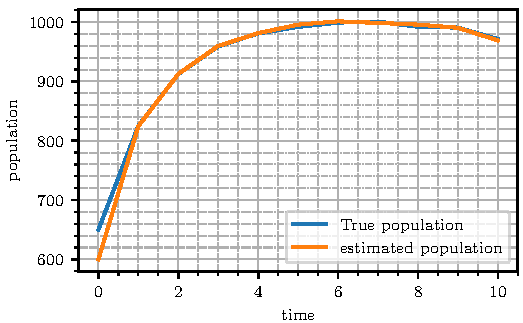
\includegraphics[scale=1.0,trim={0cm 0cm 0cm 0cm},clip]{./code/generatedPlots/q4_population.pdf}
	\caption{Q4.a: True and estimated population for 10 time steps}
	\label{fig:q4_population}
\end{figure}
Fig.~\ref{fig:q4_food} shows the true and estimated food supply for $10$ time steps.
%%%%%%%%%%%%%%%%%%%%%%% FOOD GRAPH %%%%%%%%%%%%%%%%%%%%%
\begin{figure}[!h]
	\centering
	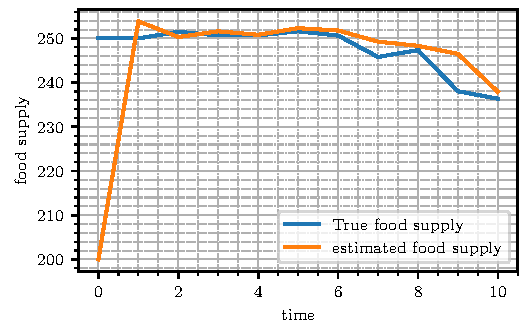
\includegraphics[scale=1.0,trim={0cm 0cm 0cm 0cm},clip]{./code/generatedPlots/q4_food.pdf}
	\caption{Q4.a: True and estimated food supply for 10 time steps}
	\label{fig:q4_food}
\end{figure}
Fig.~\ref{fig:q4_std_dev} shows the standard deviation (both $\pm$) of population and food supply estimates for $10$ time steps.
%%%%%%%%%%%%%%%%%%%%%%% STD DEV FOOD+POPULATION GRAPH %%%%%%%%%%%%%%%%%%%%%
\begin{figure}[!h]
	\centering
	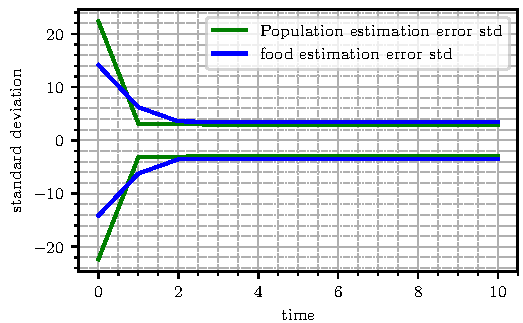
\includegraphics[scale=1.0,trim={0cm 0cm 0cm 0cm},clip]{./code/generatedPlots/q4_std_dev.pdf}
	\caption{Q4.a: Standard deviation of estimated population and food supply for 10 time steps}
	\label{fig:q4_std_dev}
\end{figure}
Fig.~\ref{fig:q4_kal_gain} shows the Kalman gains for population and food supply estimates for $10$ time steps.
%%%%%%%%%%%%%%%%%%%%%%% KALMAN GAINS GRAPH %%%%%%%%%%%%%%%%%%%%%
\begin{figure}[!h]
	\centering
	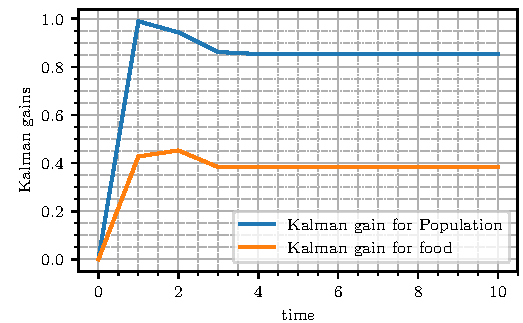
\includegraphics[scale=1.0,trim={0cm 0cm 0cm 0cm},clip]{./code/generatedPlots/q4_kal_gain.pdf}
	\caption{Q4.a: Kalman gains for population and food supply for 10 time steps}
	\label{fig:q4_kal_gain}
\end{figure}
%----------------------------------------------------------------------------------------
%	SOLUTION 4.b
%----------------------------------------------------------------------------------------
\paragraph{4.b}Fig.~\ref{fig:q4_std_dev_theoretical} shows the standard deviation (both $\pm$) of population and food supply estimates for $10$ time steps along with the steady state theoretical values (computed using covariance analysis).
%%%%%%%%%%%%%%%%%%%%%%% KALMAN GAINS GRAPH %%%%%%%%%%%%%%%%%%%%%
\begin{figure}[!h]
	\centering
	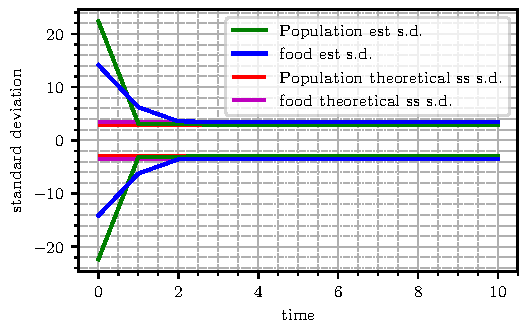
\includegraphics[scale=1.0,trim={0cm 0cm 0cm 0cm},clip]{./code/generatedPlots/q4_std_dev_theoretical.pdf}
	\caption{Q4.b: Standard deviations of population and food supply estimates for 10 time steps along with steady state(ss) theoretical values}
	\label{fig:q4_std_dev_theoretical}
\end{figure}
From Fig.~\ref{fig:q4_std_dev_theoretical}, we can see that the steady state theoretical values of standard deviations of the population and food supply estimates do not closely match with the estimated standard deviations of the same. This happens because $10$ time steps are not enough for the Kalman filter to converge closely to the theoretical value computed from covarinace analysis. We can see the improvement in 4.c.
%----------------------------------------------------------------------------------------
%	SOLUTION 4.c
%----------------------------------------------------------------------------------------
\paragraph{4.c}Fig.~\ref{fig:q4_std_dev_theoretical_1000} shows the standard deviation (both $\pm$) of population and food supply estimates for $1000$ time steps along with the steady state theoretical values (computed using covariance analysis).
%%%%%%%%%%%%%%%%%%%%%%% KALMAN GAINS GRAPH %%%%%%%%%%%%%%%%%%%%%
\begin{figure}[!h]
	\centering
	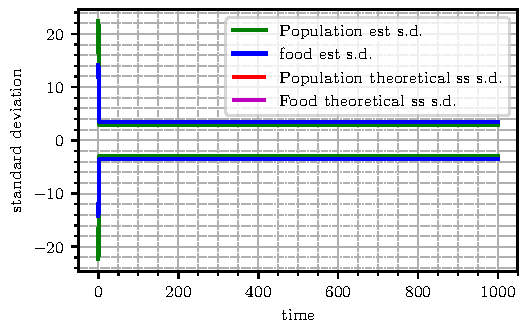
\includegraphics[scale=1.0,trim={0cm 0cm 0cm 0cm},clip]{./code/generatedPlots/q4_std_dev_theoretical_1000.pdf}
	\caption{Q4.c: Standard deviations of population and food supply estimates for 1000 time steps along with steady state(ss) theoretical values}
	\label{fig:q4_std_dev_theoretical_1000}
\end{figure}
From Fig.~\ref{fig:q4_std_dev_theoretical_1000}, we can see that the estimated standard deviations of the population and food supply converge to the steady state theoretical values as time goes by. Therefore, we can see that $1000$ time steps really improves the performance of the Kalman filter.
\paragraph{Git location of the code:} The code file has been attached as a PDF file ('script\_q4.pdf', 'kalman.pdf'). Moreover, the code can be found at\\
\url{https://github.umn.edu/dey00011/EE5251\_optimal\_filter\_estimation/tree/master/HW3/code}